Here, we demonstrate empirical performance results we have found with our
apparatus. We also attempt to highlight the underlying effects that determine
our results.

\subsection{Workload Characteristics}
We first note several key characteristics of our data corpus:
\begin{figure}[t]
    %\hspace{-10pt}
    \figuretitle{Reduction\textsuperscript{\ref{reduction_footnote}} in PLT with Varying RAM vs CPU}
    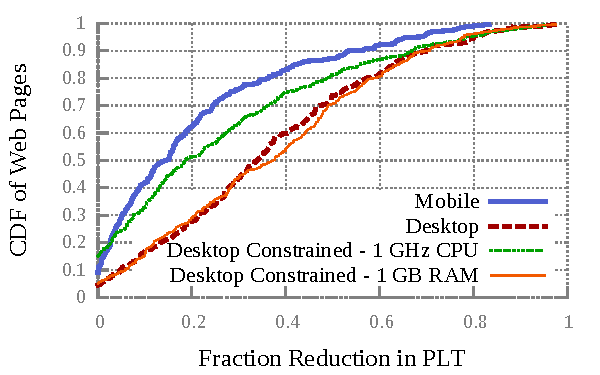
\includegraphics[width=3in]{../graphs/percent_plt_reduction/percent_reduction_linear.pdf}
    \caption[]{\label{fig:percent_reduction_linear}Reduction in page load time due to (perfect) caching is significantly less on mobile devices than desktop. Further, CPU, not RAM, is the primary resource that differentiates mobile devices from their desktop counterparts.}
\end{figure}

\textbf{Data Set}. We selected a random subset of 400 of the Alexa top 2000 URLs~\cite{alexa} and loaded their root URL (`/').
% \textbf{Cache Hit Ratio}. We experiment with two settings of cache hit ratio. To show an upper bound on how much caching can help, we evaluate the effect of a perfect (100\%) cache. We also seek to reproduce the result from Flywheel~\cite{flywheel}, by showing the difference between 20\% and 30\% cache hit ratio.
% %In their NSDI paper, Google reported that increasing the cache hit ratio by more than 50\% only increased mobile PLT by 1-2\%. Here, we seek to capture an upper bound on caching's effect on PLT. 

\textbf{Fraction of Cacheable Bytes}. Over 90\% of web pages in our workload have more than 90\% of their total bytes marked as cacheable, as shown in Figure~\ref{fig:cacheable_bytes_linear}. %This gives the initial impression that perfect caching should have a significant effect on web performance.
%Web pages generally make high use of caching between origin servers and users.

\textbf{Total Bytes}. Figure~\ref{fig:total_bytes_linear} shows the spread of web page sizes in our data set. While 95\% of web pages are under 6.8 MB, the median web page size is less than 1.2 MB.

\textbf{Initial Network Delays}. Across all requests/response pairs, the median delay between sending the request and receiving the first response byte was 50ms, with a mean of 151.17ms and standard deviation of 403.77ms.
%Initial network delays may play a role in determining the final results of our caching analysis. 
% TODO(cs): we should include this next sentence?!
%As such, we experimented with inflating all network delays by a fixed amount (100ms) to emulate what clients in an emerging market might observe. We found that the mobile results of our caching analysis were changed by 3\% in the median case (See Figure~\ref{fig:inflated_delays}).
%\arvind{this is to the original website right?  the "LAN" is confusing.}

\textbf{User Agent}. Many web pages are now optimized for mobile devices. Web
servers inspect the user agents (UA) of incoming HTTP(S) requests to deliver
customized content to the client depending on their device size and
computational resources. We ran all of our experiments twice: once where the
browsers (both desktop and mobile) advertised a mobile UA, and once where the
browsers advertised a desktop UA. We found that the differences in the results
were comparable. Here, we show only the desktop UA results to make our graphs more readable.
%\arvind{shouldn't it be that the mobile device should use mobile UA and the desktop one should use the desktop UA? the fact that the differences - as opposed to the actual values - are comparable is interesting.} \jamshed{Add slight anecdotal evidence}

\subsection{Performance Results}
As we saw in Figure~\ref{fig:cacheable_bytes_linear}, 90\% of pages are
composed of $>$90\% cacheable bytes.
If network delays were dominant and the fraction of cacheable objects on the
critical path were moderately high, one would conclude that PLT would become negligible with a perfect cache. As our model predicts however, this is not the observed outcome.

\textbf{Caching Doesn't Significantly Reduce Mobile PLT}.
We reproduced Flywheel's result in our controlled environment by emulating cache hit ratios of 20\% and 30\%. As shown in Figure~\ref{fig:partial_cache_linear}, we found that increasing the hit ratio by 10 percentage points had negligible effects on mobile page load time. Consistent with the reported Flywheel result, we observed only a 1\% reduction in PLT in the median case.
With a {\em perfect} cache (Figure~\ref{fig:percent_reduction_linear}), our mobile device gains only a 13\% PLT reduction
in the median case, while its desktop counterpart sees a PLT reduction of
34\%.

\begin{figure}[t]
    %\hspace*{-0.11in}
    \figuretitle{Reduction\textsuperscript{\ref{reduction_footnote}} in PLT with Varying CPU Speeds}
    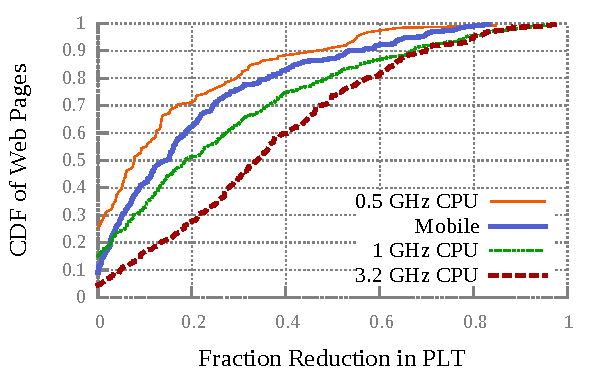
\includegraphics[width=3in]{../graphs/percent_plt_reduction/percent_reduction_linear_CPU_comparison.pdf}
    \caption[]{\label{fig:plt_cpu_comparison}Slower CPU speeds cause increasingly diminished benefits from (perfect) caching.}
\end{figure}
{\bf Limited RAM Does Not Affect Computational Delays.}
% Dialogue: Is it RAM or CPU? -> Explain RAM figure.
% Conclusion: not RAM, but CPU.
It is possible that either limited RAM, or limited CPU would increase computational delays on the critical path.
Here, we seek to isolate which of these resources plays a larger role.

A typical mobile device in the global market today has a 1 GHz processor and 1 GB of RAM~\cite{mobile-stats}. We emulate these conditions and isolate computational resources with virtual machines that were constrained by different resources (using VirtualBox to either set a limit on memory usage or emulate a slower CPU clock speed).
With `Mobile' and (unconstrained) `Desktop' as baselines, Figure~\ref{fig:percent_reduction_linear} presents a stark contrast between these resource constraints:
our CPU constrained VM (`Constrained - 1 GHz CPU') behaves very
similarly to our tablet (`Mobile'), while our RAM constrained VM (`Constrained - 1 GB RAM') is more closely aligned with the `Desktop' results.
From this we conclude that CPU, not RAM, plays the larger role in determining the performance improvements from caching.

\stepcounter{footnote}
\stepcounter{footnote}

{\bf Slow CPU Speeds Increase Computational Delays.}
% We know that CPU is the bottleneck, so we look into varying the CPU.
Now that we have isolated CPU as the bottleneck resource, we seek to measure
the extent of its impact. In terms of our model, we already know that slower
CPUs should incur higher computational delays, but here we seek to understand
the empirically observed ratios of $C:N$ (as opposed to the hypothetical,
predicted ratios in Figure~\ref{fig:whatif}).
\footnotetext{\label{reduction_footnote}The fraction reduction in PLT for a web page is defined as\\(Original PLT - PLT with a perfect cache) / (Original PLT).}
In Figure~\ref{fig:plt_cpu_comparison}, we observe that, as predicted,
as we throttle CPU constraints, perfect caching has noticeably smaller effects on PLT. % TODO(cs): point out what the ratio of C:N is.

{\bf The Marginal Benefits of Caching Sharply Decrease.}
Figure~\ref{fig:ratio_linear_comparison} illustrates that for each 10 percentage point increase in cache hit ratio, there is only
a 1 percentage point decrease in mobile page load time.
That is, there is a sharply diminishing marginal performance gain for 
every additional byte that is cached.
This experimental evidence supports our model:
although we do not directly measure the critical path (since WProf is not currently available for mobile browsers), it appears that the fraction of cacheable bytes on the critical path ($K$) is
significantly smaller than the fraction of cacheable byes {\it not} on
the critical path.

%\colin{Can cut this if we need space}
%Consistent with the results found in WProf~\cite{wang2013demystifying}, our results show that reduction in PLT is not proportional to number of bytes cached. Although we do not measure the critical path precisely (since WProf is not currently available on mobile browsers), we believe that a low value of $K$, and a relatively high ratio of $C:N$ explain our observations.
% 
%We hypothesize that the delays of objects on the critical path are also elongated by a constrained CPU.
%These factors contribute to a longer critical path that is prone to the benefits of caching.
%\arvind{above discussion is not clear; and it is probably the most critical observation that we need to communicate precisely}

%\footnotetext{The fraction reduction in PLT for a web page is defined as\\
%(Original PLT - PLT with a perfect cache) / (Original PLT)}

\subsection{Data Validation}
\label{subsec:validation}
We made several efforts to sanity check our results~\cite{sanity-checks}. To
mitigate non-determinism, we compared the status codes of all objects loaded
in the browser from both original and perfect/partial cache benchmarks. We
filtered out about 9\% of web pages in our 400 URL data set in cases where
there were a high number of 404 error codes due to non-deterministic requests
without responses in the WPR archive. The figures we present show only these
91\% of web pages that passed our non-determinism filter.

As the ratio of cached to non-cached bytes increases in a web page, we expect page load time to be less than or equal to that of its non-cached counterpart. As seen in Figure~\ref{fig:ratio_linear_comparison}, there is a positive correlation between the fraction of cached bytes and the reduction in PLT, albeit asymptotic.
However, due to variance in PLT (discussed in~~\S\ref{known_limitations}), we
see in Figure~\ref{fig:percent_reduction_linear} that
{\footnotesize$\sim$}10\% of web pages perform worse when cached, as
indicated by the data points to the left of \texttt{X = 0}.
\begin{figure}[t]
    %\hspace{-10pt}
    \figuretitle{Ratio of Fraction Cacheable Bytes to PLT}
    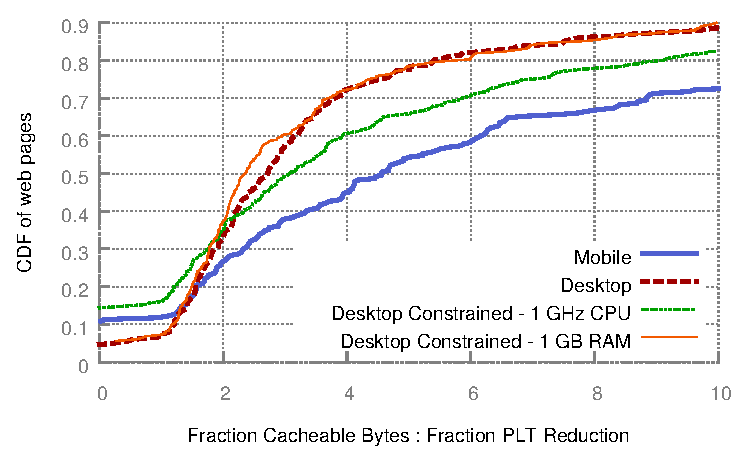
\includegraphics[width=3in]{../graphs/ratio_bytes_to_reduction/ratio_linear_comparison.pdf}
    \caption[]{\label{fig:ratio_linear_comparison}As the percentage of cacheable bytes in a web page increases, the reduction in page load time due to caching increases. However, for each additional percentage cached, there is less than a percentage reduction in page load time.}
\end{figure}
